\chapter{Optical Transparent Networks Dimensioning}
\label{chapter2}

The scope of this chapter resides on the elaboration of a state-of-the-art review relatively to optical transport networks. This chapter is composed of 5 subsections, the first \ref{networkArchitecture} provides a generic description on optical transport networks and addresses the main constituting  components, the second \ref{networkTopologies} refers and provides a brief description on the different topologies in a network, the third \ref{CapitalExpanditure} is an approach on the various methods of calculating the \gls{capex} of a network and the last two describe both the reference and the realistic networks considered for the various types of dimensioning processes, \ref{referenceNetwork} and \ref{realisticNetwork}, respectively.

\section{Network Architecture}
\label{networkArchitecture}

In the modern telecommunications era, networks are a vast and highly multidisciplinary field of study as it shall be seen further along this dissertation. As it was mentioned in the previous chapter, traffic requirements have been growing unbelievably fast in the last few decades and so an efficient and well structured network becomes a priority of even greater importance over time once the direct consequence is the minimization of required network components, thus, lowering the respective \gls{capex} of the network. \par In the transparent transport mode, which will be the transport mode studied, signals remain in the optical domain from their source till the destination node, traveling in a defined route through one or more optical channels that together constitute a high-bandwidth end-to-end circuit, i.e., a lightpath \cite{1255431}. Therefore, a single-hop grooming scheme is used as intermediate nodes do not perform wavelength conversions and so the requests must be assigned with the same wavelength on all the links of the used path \cite{Sridharan:2004:BAN:987232.987247}. This is known as the wavelength continuity constraint and implies that the utilization of the same wavelength channels is restricted to the client signals with the same endpoints \cite{RuiMoraisPhD}. Also in this transport mode the so called electro-optic bottleneck is eliminated as this method allows information transfer rates to reach closer values to those allowed by optical devices, which are significantly beyond the rates achievable in an \gls{o-e-o} network \cite{664268}. Electrical regeneration is also not present, and as such the quality of the optical signals degrade as they traverse the optical components along the route limiting the maximum transmission length of the signals in the optical domain without regeneration \cite{RuiMoraisPhD}. Regarding the network economic aspects, the dimensioning of a telecommunications network involves identifying the required resources and their respective quantities \cite{estimatingCapex}. As both setting up and operating large telecommunications infrastructures require large amounts of money any network investment must be carefully evaluated \cite{anpinto2}. These costs can be divided into two major branches: the \gls{capex} and the \gls{opex}. The first will be analyzed more closely during this dissertation and can be sub-divided into the cost of buying and installing the equipment as well as setting up the infrastructures and the second represents an expense a network company incurs through its normal operations, which can include rent, inventory costs, insurance, and funds allocated for research and development \cite{anpinto}\cite{OPEX}.

\begin{figure}[H]
  \begin{center}
    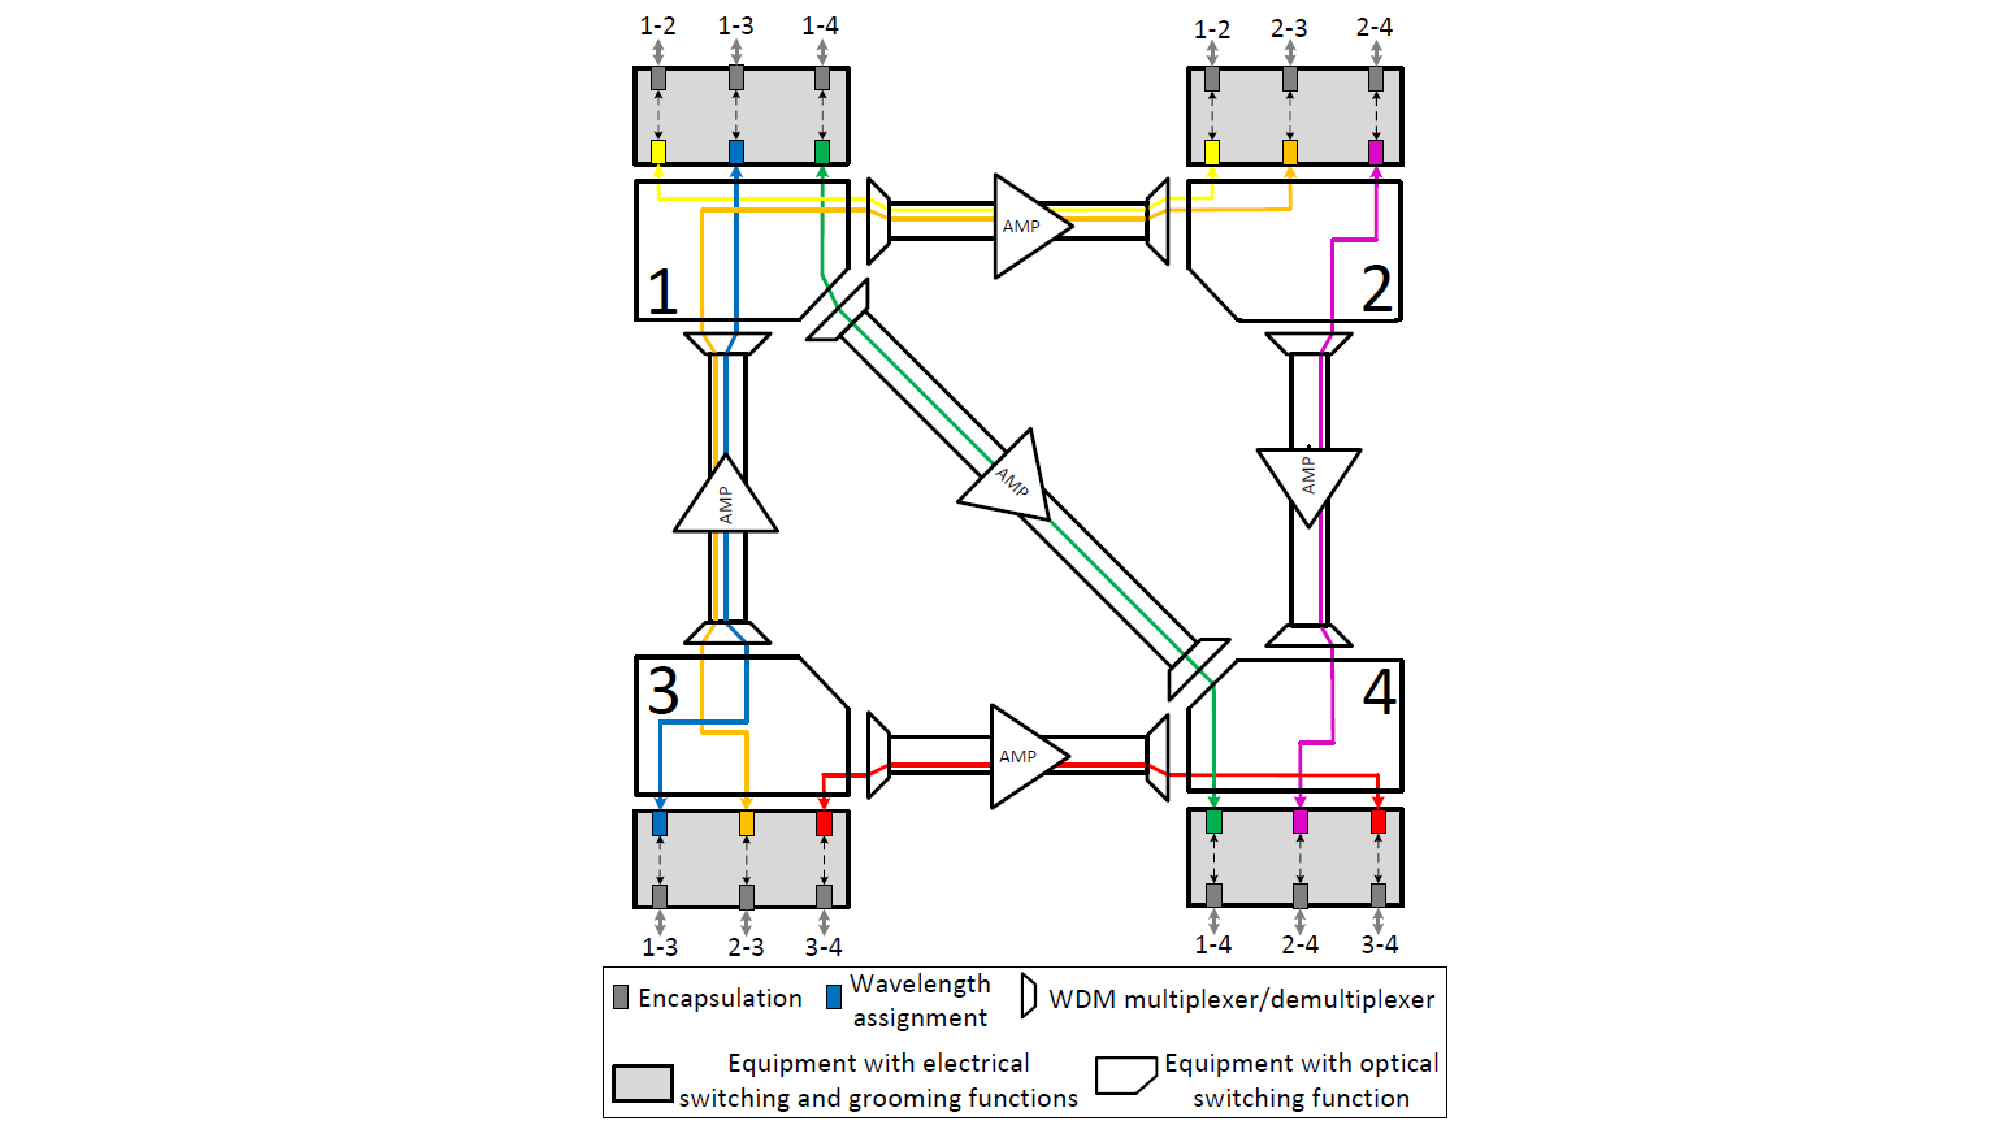
\includegraphics[width=1\textwidth]{fig/logos/transparentNode.pdf}
    \caption{Example of an all-optical network with 4 nodes \cite{RuiMoraisPhD}.}
  \end{center}
  \label{exampleTransparentNetwork}
\end{figure}

Above in figure \ref{exampleTransparentNetwork} an example of a four nodes all-optical network is shown where a single-hop grooming technique is used and O-E-O conversions only happen at end nodes. Also, the grooming of client signals is restricted to services with the same end-points \cite{RuiMoraisPhD}. 
\clearpage 
An optical transport network can be seen as set of bidirectional links connecting nodes \cite{RuiMoraisPhD}. Links and nodes are interconnected through compatible interfaces in order to form a topology. Therefore, a network topology can be described as the arrangement of nodes and links, and are usually represented as a graph. 

\subsection{Links}
Physical point-to-point connections ensured by transmission systems between a pair of adjacent nodes, thus guaranteeing the transmission of \gls{wdm} signals between them \cite{TiagoEsteves}. Links can be composed by one or more transmission systems where each one usually comprises one pair of unidirectional optical fibers ensuring a bidirectional connection between the nodes \cite{RuiMoraisPhD}. The optical fiber is the medium where the optical signal is transmitted and is capable of transporting data on wavelengths \cite{ramaswami}. In networks capable of allowing the transiting traffic to remain in the optical domain, as it is the case, it must be considered another important property of the transmission systems which is the optical reach, the maximum distance a signal can be transmitted in the optical domain before it degrades to a level where it is required optical amplification of the signal, in order to allow a correct detection of the same in the receptor \cite{SimmonsJane2008}. The distance between each amplification stage is typically denominated span.

\begin{figure}[H]
  \label{cisco}
  \begin{center}
    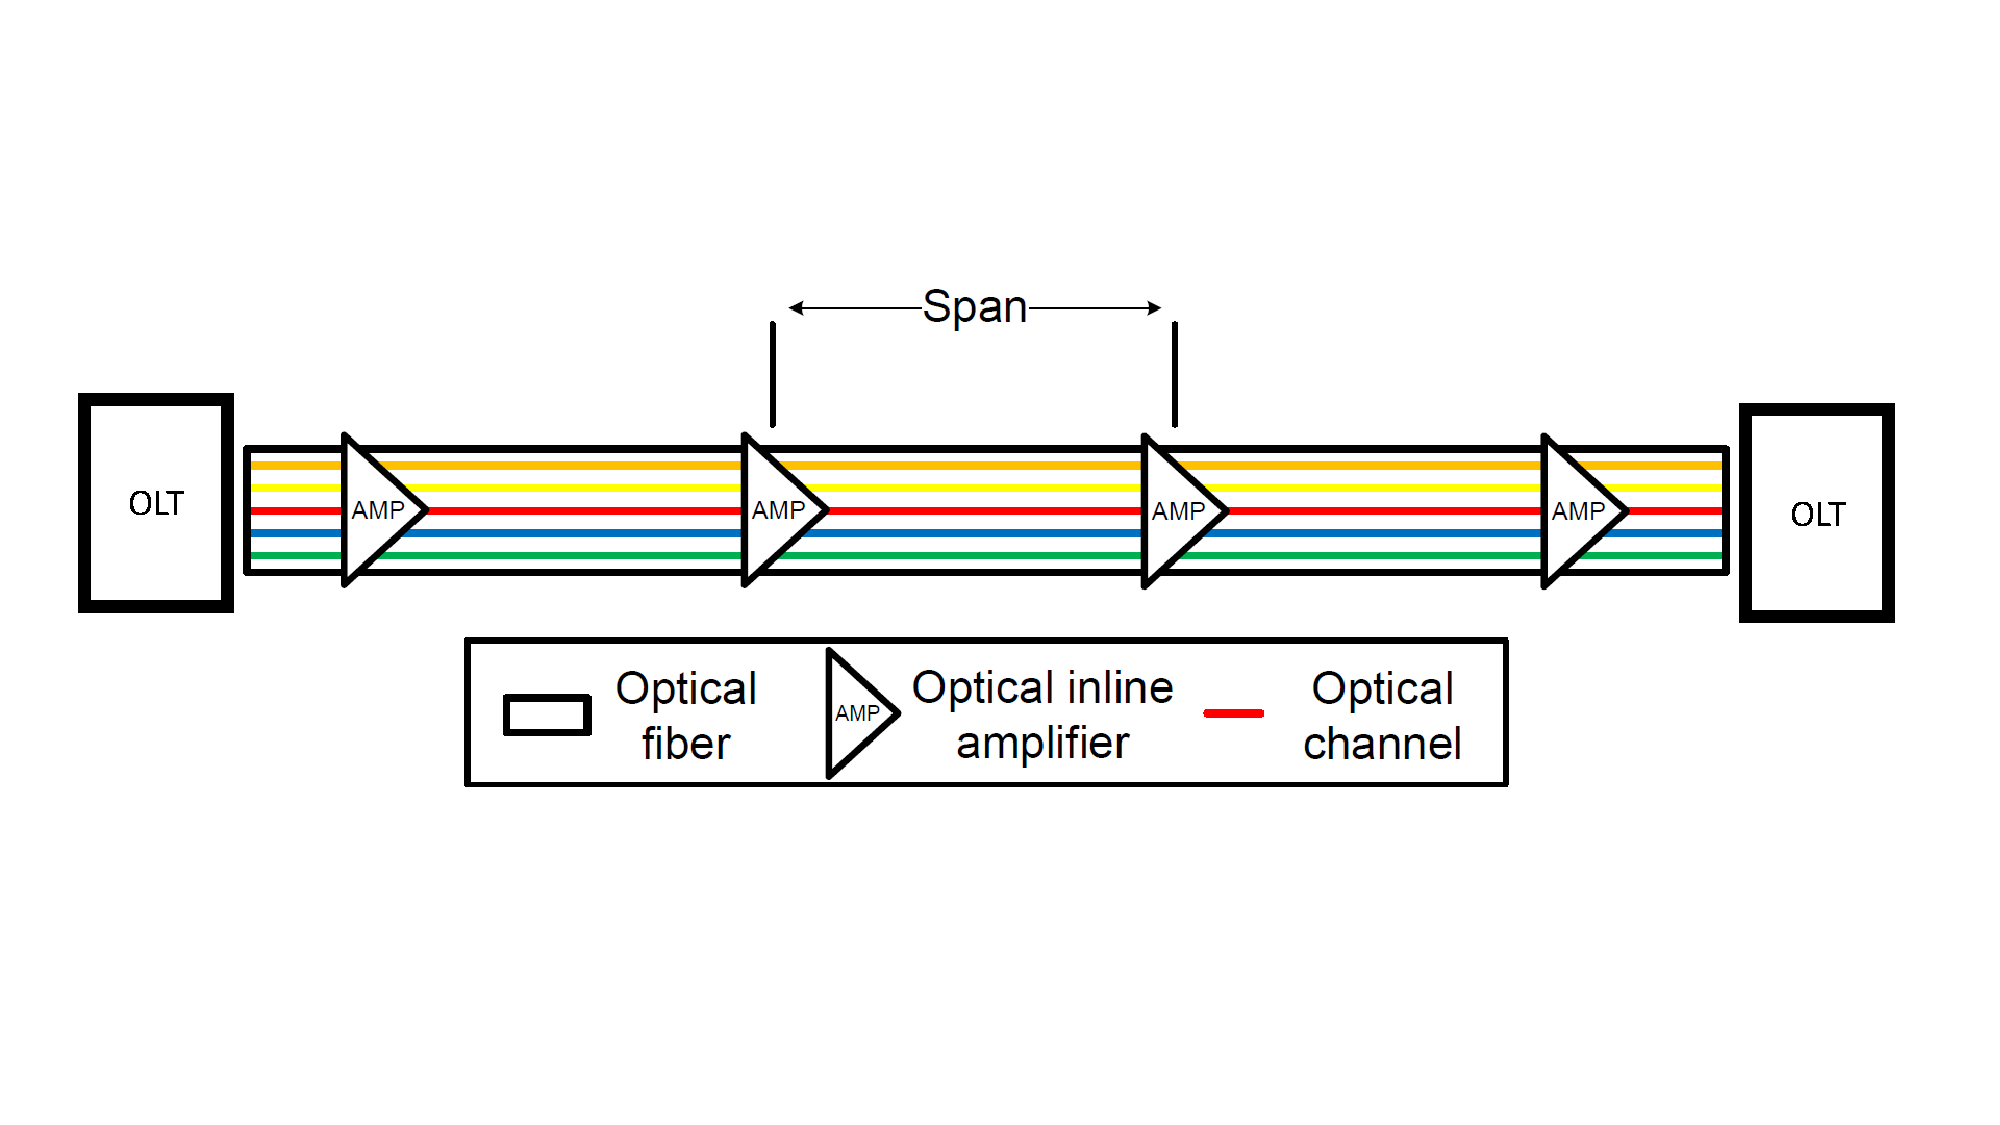
\includegraphics[width=0.7\textwidth]{fig/logos/link.pdf}
    \caption{Schematic of a link containing an optical fiber, inline optical amplifiers and OLT terminals \cite{RuiMoraisPhD}.}
  \end{center}
\end{figure}

\subsection{Nodes}

Nodes are multirack systems that usually perform six main functions being them as it follows: encapsulation, electrical switching, deterministic or statistical multiplexing (grooming), wavelength assignment, optical switching and finally optical multiplexing. All of these tasks require a substantial amount of hardware making the nodes one of the most expensive components of the network \cite{anpinto}. Moreover, as in all-optical networks the transiting traffic can potentially remain in the optical domain from source to destination, crossing through the node rather than be electronically processed, technology had to be developed in order to enable this so called optical bypass. This process would imply a significant reduction in the amount of required nodal electronic equipment, thus reducing the monetary value needed to implement it. The three major network elements that are capable of optical bypass are the \gls{oadm}, the multi-degree OADM and the all-optical switch \cite{SimmonsJane2008}. In optical networks, nodes consist mainly of three different blocks: modules, shelves and racks. The independent modules are attached to shelves in order to allow backplane communication and possess a required number of ports and other different components that perform functions on both the optical and the electrical domains, such as, optical and electrical switching, encapsulation, grooming and wavelength assignment. Regarding the shelves they provide a common infrastructure to the modules and are attached into racks which consist in frames for mounting multiple shelves and provide power and cooling to the system \cite{RuiMoraisPhD}. Ports can be defined as bidirectional optical connectors used to interconnect two modules using a pair of fibers. Each type of module occupies a given number of slots, which are the minimum unit space in a shelf and some of those slots in the shelf are reserved for the control modules which are required for operation, administration, and management tasks of the system.
 
 \begin{figure}[H]
  \label{cisco}
  \begin{center}
    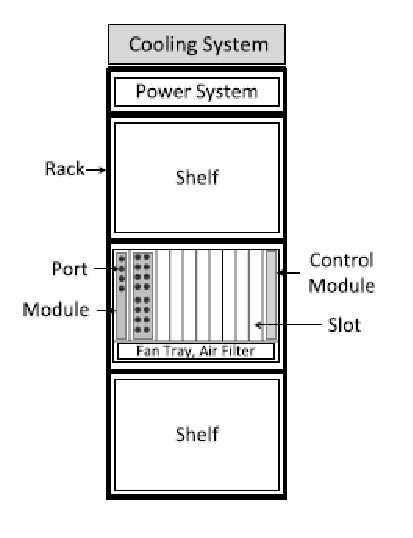
\includegraphics[width=0.40\textwidth]{fig/logos/node.pdf}
    \caption{Schematic of a node structure containing modules, shelves and a rack. \cite{6515886}.}
  \end{center}
\end{figure}



\clearpage

\section{Network Topologies}
\label{networkTopologies}
% 1.7 Network Design and Planning ---> Jane Simmons

\subsection{Physical Topology}

The pattern that represents and characterizes the layout of an optical network, i.e., the physical disposition of nodes and the connections between them. A physical network topology can be modeled as a graph which is a mathematical structure made of a set of vertices, representing nodes, and a set of edges, representing links. Graphs are usually represented pictorially using dots and arcs to represent vertices and edges, respectively, or by adjacency matrices. An adjacency matrix is a matrix containing only zeros and ones and where the position of the ones specify which vertices are directly connected to which other vertices \cite{anpinto2}.  

\subsection{Logical Topology}

Represents how the components of an optical network are connected. Each node may be either optically connected to each other, or only optically connected to adjacent or suitable nodes. This leads to a situation where different transport modes are possible to exist, namely, the opaque, the transparent and the translucent \cite{Vasco}. In this dissertation the focus will be on the transparent transport mode. Likewise the physical topology, previously referred, it can also represented as a graph or through adjacency matrices. %On the other hand, the logical topology can also represent how the flow of traffic occurs in the network, either in terms of traffic requests or logical links \cite{TiagoEsteves}.  


\section{Capital Expenditure Estimation}
\label{CapitalExpanditure}

In this section is intended to provide the general equations used in order to make CAPEX calculations. As networks are mainly comprised of nodes and links in order to calculate the total network cost it has to be considered the sum of these two components costs. The \gls{capex} value of a network, $C_C$, in monetary units (e.g. euros, or dollars), can be expressed by equation \ref{Capex_heuristic}

\begin{equation}
C_C = C_L + C_N
\label{Capex_heuristic}
\end{equation}

\noindent
where

\begin{itemize}
\item{$C_L$				$\rightarrow$	Links setup cost in monetary units (e.g. euros, or dollars)}
\item{$C_N$				$\rightarrow$	Nodes setup cost in monetary units (e.g. euros, or dollars)}
\end{itemize}

Below in this section are proposed and described the models used to calculate the CAPEX of the network. These calculations are made based on the transparent transport mode without survivability case.

\subsection{Links Cost}
\label{linksCost_}

 First lets focus on the cost of the links part, $C_L$, in monetary units (e.g. euros, or dollars). Links can be implemented with one or more transmission systems, whose cost is directly impacted by three major components, the costs regarding the \gls{olt}, the optical regeneration stages and the optical fiber. However, this last component can be discarded as it usually appears as an operational expense instead of a capital expenditure since it is commom practice in the telecommunications area for operators to lease fiber-optic cables instead of installing them \cite{anpinto}. In this dissertation each existent link is considered to possess just one bidirectional transmission system. %It is also important to stress the fact that for calculation purposes that each link is considered to be unidirectional in such a way that the combination of a pair of links creates a bidirectional connection between nodes. This makes it possible to dimension transport networks without having obligatory symmetric traffic between pairs of nodes.
 

%The following equation \ref{analytical_linkCosts_bidirectional} would be used if we were considering bidirectional links but as previously stated we are using unidirectional links to perform these calculations so the previous equation must be updated in a way that all its terms must be divided by 2 resulting in equation \ref{analytical_linkCosts_unidirectional}.
\vspace{11pt}

In order to calculate the cost of the links, we can use use equation \ref{Capex_Link}.

\begin{equation}
C_L = \sum_{i=1}^N \sum_{j=i+1}^N L_{ij} \bigg( 2 \gamma_0^{OLT} + 2 \gamma_1^{OLT} W_{ij} + 2 N^R_{ij} c^R \bigg)
\label{Capex_Link}
\end{equation}

\noindent
where
\begin{itemize}
\item{$i$               $\rightarrow$   Index for start node of a physical link}
\item{$j$               $\rightarrow$   Index for end node of a physical link}
\item{$N$				$\rightarrow$	Total number of nodes, N $\in \mathbb{N}$}
\item{$L_{ij}$			$\rightarrow$	Binary variable indicating if link between the nodes $i$ and $j$ is used, $L_{ij} \in {0, 1}$}
\item{$\gamma_0^{OLT}$	$\rightarrow$	OLT base cost in monetary units (e.g. euros, or dollars)}
\item{$\gamma_1^{OLT}$	$\rightarrow$	OLT optical channels linear cost factor in monetary units (e.g. euros, or dollars)}
\item{$W_{ij}$          $\rightarrow$   Total number of optical channels in link $i$ $j$}
\item{$N^R_{ij}$    	$\rightarrow$	Number of optical amplifiers in link $i$ $j$}
\item{$c^R$				$\rightarrow$	Unidirectional optical amplifiers cost in monetary units (e.g. euros, or dollars)}
\end{itemize}

\vspace{11pt}
The number of amplifiers for each link can be calculated by equation \ref{Capex_amplifiers}

\begin{equation}
N^R_{ij} = \left(\left\lceil\frac{len_{ij}}{span}\right\rceil-1\right)
\label{Capex_amplifiers}
\end{equation}

\vspace{11pt}
\noindent
where the variable $len_{ij}$ is the length of link $ij$ in kilometers and the $span$ is the distance between amplification stages, also in kilometers \cite{anpinto2}.

%This is where the various methodologies will diverge, once the average number of optical channels will depend directly of $<h>$, the average number of hops per demand, and  of $D$ which is the number of unidirectional demands processed by the network. While the analytical method uses approximated values for this parameters the ILPs and heuristics have access to all the information and as such will utilize the optimal values found by the algorithms.

\subsection{Nodes Cost}
\label{nodesCost_}

Regarding the nodes part of the costs, in transparent network nodes it is necessary to consider both the optical and the electrical parts, as it can be seen below in figure \ref{opticalElectricalNode}. The channels that just go through the node are switched in the optical domain and the channels that are local to the node are processed in the electrical domain, with the switching being performed in the wavelength-domain \cite{anpinto2}. So, as the nodes have an electrical part, the \gls{exc}, and an optical part, the \gls{oxc}, it becomes obvious that the cost of the nodes, $C_N$, is given by the sum of these two parts, thus, obtaining the equation \ref{Capex_Node_heuristic}
\vspace{11pt} 

\begin{equation}
C_N = C_{EXC} + C_{OXC}
\label{Capex_Node_heuristic}
\end{equation}

\noindent
where

\begin{itemize}
\item {$C_{EXC}$        $\rightarrow$   Electrical node cost in monetary units (e.g. euros, or dollars)}
\item {$C_{OXC}$        $\rightarrow$   Optical node cost in monetary units (e.g. euros, or dollars)}
\end{itemize}

\begin{figure}[H]
  \begin{center}
    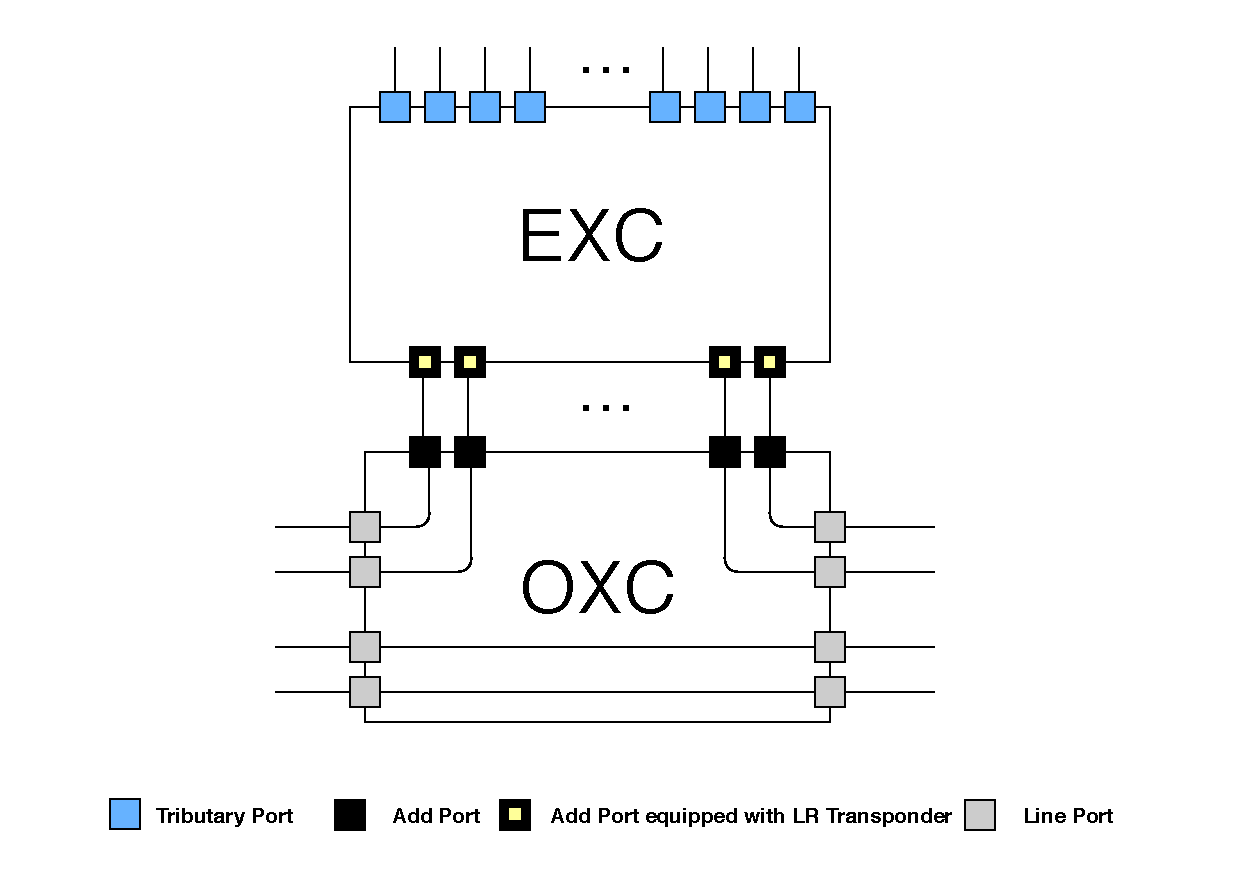
\includegraphics[width=0.7\textwidth]{fig/logos/nodeScheme.pdf}
    \caption{Electrical and optical node structure.}
  \end{center}
  \label{opticalElectricalNode}
\end{figure}


The electric cost is than the sum of the fixed cost of the electrical connection with the total cost of all the electric ports. Therefore, the electric cost in monetary units (e.g. euros, or dollars), $C_{EXC}$, is given by equation \ref{Capex_Node_EXC} \cite{TiagoEsteves}.

\begin{equation}
C_{EXC} = \sum_{n=1}^{N} N_{exc,n} \left( \gamma_{e0} + \sum_{c=-1}^B \gamma_{e1,c} P_{exc,c,n} \right)
\label{Capex_Node_EXC}
\end{equation}

\noindent
where
\begin{itemize}
\item{$N$				$\rightarrow$	Total number of nodes, N $\in \mathbb{N}$}
\item{$N_{exc,n}$		$\rightarrow$	Binary variable indicating if node $n$ is used, $N_{exc,n} \in {0, 1}$}
\item{$\gamma_{e0}$ 	$\rightarrow$	EXC base cost in monetary units (e.g. euros, or dollars)}
\item{$\gamma_{e1,c}$	$\rightarrow$	EXC port cost in monetary units (e.g. euros, or dollars) with bit-rate $B$ and with a given transceiver reach}
\item{$P_{exc,c,n}$	    $\rightarrow$	Number of ports of the electrical switch of node n}
\item{$B$           	$\rightarrow$	A natural number corresponding to the maximum index of short-reach ports, see table \ref{table_bitrate}}
\end{itemize}

\begin{table}[h!]
\centering
\begin{tabular}{|c|c|}
  \hline
  Index & Bit rate \\
 \hline
  -1 & 100 Gbits/s line bit-rate (long-reach port) \\
  0 & 1.25 Gbits/s tributary bit-rate (short-reach port) \\
  1 & 2.5 Gbits/s tributary bit-rate (short-reach port) \\
  2 & 10 Gbits/s tributary bit-rate (short-reach port) \\
  3 & 40 Gbits/s tributary bit-rate (short-reach port) \\
  4 & 100 Gbits/s tributary bit-rate (short-reach port) \\
  \hline
\end{tabular}
\caption{Table containing indexes and the corresponding bit rates.}
\label{table_bitrate}
\end{table}

%%%%%%%%%%%%%%%%%%%%%%%%%%%%%%%%%%%%%%%%%%%%%%%%%%%%%%%%%%%%%%%%%%%%%%%%%%%

The following equation \ref{EXC_pexc1_transparent} refers to the number of short-reach ports of the electrical switch with bit-rate $c$ in node $n$, $P_{exc,c,n}$, i.e. the number of tributary ports with bit-rate $c$ in node $n$, \cite{TiagoEsteves}. It can be calculated as

\begin{equation}
P_{exc,c,n} = \sum_{d=1}^{N} D_{nd,c}
\label{EXC_pexc1_transparent}
\end{equation}

\noindent
where $D_{nd,c}$ are the client demands between nodes $n$ and $d$ with bit rate $c$.\\

In this case there is the following particularity:
\begin{itemize}
  \item When $n$=$d$ the value of client demands is always zero, i.e, $D_{nn,c}=0$
\end{itemize}

On the other hand, the equation \ref{EXC_pexc2_transparent} refers to the number of long-reach ports of the electrical switch with bit-rate -1 in node n, $P_{exc,-1,n}$, i.e. the number of add ports of node n, \cite{TiagoEsteves}. It can be calculated as

\begin{equation}
P_{exc,-1,n} = \sum_{j=1}^{N} \lambda_{nj}
\label{EXC_pexc2_transparent}
\end{equation}

\noindent
where $\lambda_{nj}$ is the number of optical channels between node $n$ and node $j$.

\vspace{11pt}

In relation to the optical part, $C_{oxc}$, once again the optical cost is the sum of the fixed cost of the optical connection with the total cost of all the optical ports. Therefore the optical cost in monetary units (e.g. euros, or dollars), $C_{OXC}$, is given by equation \ref{Capex_Node_OXC} \cite{TiagoEsteves}.

\begin{equation}
C_{OXC} = \sum_{n=1}^{N} N_{oxc,n} \bigg( \gamma_{o0} + \gamma_{o1} P_{oxc,n} \bigg)
\label{Capex_Node_OXC}
\end{equation}

\noindent
where
\begin{itemize}
\item{$N$				$\rightarrow$	Total number of nodes, N $\in \mathbb{N}$}
\item{$N_{oxc,n}$		$\rightarrow$	Binary variable indicating if node $n$ is used, $N_{oxc,n} \in {0, 1}$}
\item{$\gamma_{o0}$ 	$\rightarrow$	OXC base cost in monetary units (e.g. euros, or dollars)}
\item{$\gamma_{o1}$ 	$\rightarrow$	OXC optical channels linear traffic cost in monetary units (e.g. euros, or dollars) }
\item{$P_{oxc,n}$	    $\rightarrow$	Number of ports of the optical switch of node n}
\end{itemize}

\vspace{11pt}

The following equation refers to the number of ports in the optical switch of node n, $P_{oxc,n}$, i.e. the number of line ports and the number of adding ports of node n \cite{TiagoEsteves}. It can be calculated as

\begin{equation}
P_{oxc,n} = P_{line,n} + P_{add,n}
\label{OXC_poxc_transparent2}
\end{equation}

\noindent
which is equivalent to  the equation \ref{OXC_poxc_transparent} expressed below.\\

\begin{equation}
P_{oxc,n} = \sum_{j=1}^{N} f_{nj}^{od} + \sum_{j=1}^{N} \lambda_{nj}
\label{OXC_poxc_transparent}
\end{equation}

\noindent
where $f_{nj}^{od}$ refers to the number of line ports for all demand pairs (od) and $\lambda_{nj}$ refers to the number of add ports.\\
\clearpage

\subsection{Capital Expenditure Models}

The values obtained for the \gls{capex} of the tested networks will most probably vary for the exact same traffic scenario considering the model used (analytical, ILP or heuristic) since the calculated values for variable $P_{exc,c,n}$ and $P_{oxc,n}$ will always depend upon the mode of transport used and on the routing and grooming strategies, which differ according to the model used. In order to make these calculations, it will also be needed to take into account the costs of the equipment used, which are presented in table \ref{table_cost}, and will represent the steady variables of the problem.




\begin{table}[H]
\centering
\begin{tabular}{| c | c | c |}
 \hline
  & Symbol & Cost \\
 \hline
 OLT base cost & $\gamma_0^{OLT}$ & 15 000 \euro \\
 OLT optical channels linear cost factor & $\gamma_1^{OLT}$ & 5 000 \euro \\
 Unidirectional optical amplifier & $c^R$ & 2 000 \euro \\
 EXC base cost & $\gamma_{e0}$ & 10 000 \euro \\
 OXC base cost & $\gamma_{o0}$ & 20 000 \euro \\
 Long reach transponder & $\gamma_{e1}$ & 100 \euro /Gbit/s\\
 EXC traffic linear factor cost & $\gamma_{e2}$ & 100 \euro/Gbit/s\\
 OXC optical channels linear traffic cost & $\gamma_{o1}$ & 2 500 \euro /port \\
 \hline
\end{tabular}
\caption{Table of costs used to calculate the CAPEX \cite{anpinto}.}
\label{table_cost}
\end{table}


\subsubsection{Analytical Model}
\label{anal}
The analytical approach is used when a statistical approximation is required not existing the need for exact and precise values. This estimation becomes useful for cases where there is lack of some information, for example the number of demands to process or the topology of the network, or when the routing and/or grooming processes are unknown. %Having that said, through equations \ref{optical_channels} and \ref{demands} it becomes possible to calculate an approximated value for the remaining unknown variables in this case . The average number of optical channels \cite{TiagoEsteves}, $<w>$, as

\vspace{11pt}
In this section the calculations are made in an analytical way in order to get a different point of view while expecting similar results. Having this said, the CAPEX in monetary units, $C_C$ is again given by the equation \ref{Capex_heuristic}.\\ \\

For this calculation first let's focus on the cost of the links. Where to calculate the cost of the Links, $C_L$, it is used the equation \ref{analytical_linkCosts}
\vspace{11pt}

\begin{equation}
C_L = \left(2 L \gamma_0^{OLT}\right) + \left(2 L \gamma_1^{OLT} <w>\right) + \left(2 N^R c^R\right)
\label{analytical_linkCosts}
\end{equation}

\vspace{11pt}
\noindent
\clearpage
where
\begin{itemize}
\item{$\gamma_0^{OLT}$	$\rightarrow$	OLT base cost cost in monetary units (e.g. euros, or dollars)}
\item{$L$				$\rightarrow$	Number of bidirectional links}
\item{$\gamma_1^{OLT}$	$\rightarrow$	OLT optical channels linear cost in monetary units (e.g. euros, or dollars)}
\item{$<w>$             $\rightarrow$   Average number of optical channels}
\item{$N^R$				$\rightarrow$	Total number of unidirectional optical amplifiers}
\item{$c^R$				$\rightarrow$	Unidirectional optical amplifiers cost in monetary units (e.g. euros, or dollars)}
\end{itemize}

\vspace{11pt}
Looking at the equation \ref{analytical_linkCosts} it becomes obvious that practically all the values of the variables used are known, only missing the number of optical amplifiers and the average number of optical channels \cite{anpinto2}.\\

Through the equation \ref{amplifiers} we can calculated the number of optical amplifiers, $N^R$, as

\begin{equation}
N^R = \sum\limits_{l=1}^L\left(\left\lceil\frac{len_l}{span}\right\rceil-1\right)
\label{amplifiers}
\end{equation}

\vspace{11pt}
\noindent
where $len_l$ is the length of link $l$ and $span$ is the distance between amplifiers, again assumed to be of 100 km \cite{anpinto2}.\\

\vspace{11pt}
The average number of optical channels can be calculated as it follows, through equation \ref{optical_channels} \cite{TiagoEsteves}.

\begin{equation}
<w> = \left( \frac{\lceil D \vspace{2pt} <h> \rceil}{L_u} \right) \left( 1 + <k>\right)
\label{optical_channels}
\end{equation}

\noindent
where $D$ is the number of unidirectional demands, $L_u$ is the number of unidirectional links and $<k>$ is the survivability coefficient.
And finally the number of unidirectional demands can be calculated as

\begin{equation}
D = \left(\frac{1}{2}\right) \left( 1 + \xi \right) \left(\frac{T_1}{\tau}\right)
\label{demands}
\end{equation}

\noindent
where $\xi$ is the grooming coefficient, $T_1$ is the total unidirectional traffic and $\tau$ is the line bit rate, assumed to be 100 Gbit/s \cite{TiagoEsteves}.\\

Taking into account the particularities of the transparent transport mode it will be assumed the following values:
\begin{itemize}
  \item $\xi$ = 1.25
  \item $<k>$ = 0 (there is no survivability)
\end{itemize}

It will be assumed that the grooming coefficient has value 1.25 and that the survivability coefficient is zero because it is not considered survivability.

\vspace{11pt}
Relatively to the cost of the nodes, it can be expressed as in equation \ref{Capex_Node_heuristic}, being the electrical cost of the nodes, $C_{exc}$, given by equation \ref{analytical_electricalCost}.

\begin{equation}
C_{exc} = N \left( \gamma_{e0} + \left( \gamma_{e1} \tau <P_{exc}> \right) \right) + \gamma_{e2} \ P_{trib}
\label{analytical_electricalCost}
\end{equation}

\vspace{11pt}
\noindent
where:
\begin{itemize}
\item{$N$			$\rightarrow$	Number of nodes}
\item{$\gamma_{e0}$	$\rightarrow$	EXC base cost in monetary units (e.g. euros, or dollars)}
\item{$\gamma_{e1}$	$\rightarrow$	Long reach transponder cost in monetary units (e.g. euros, or dollars)}
\item{$\gamma_{e2}$	$\rightarrow$	EXC traffic linear factor cost in monetary units (e.g. euros, or dollars)}
\item{$\tau$		$\rightarrow$	Line bit rate}
\item{$<P_{exc}>$   $\rightarrow$   Average number of ports of the electrical switch}
\item{$P_{trib}$    $\rightarrow$   Total number of tributary ports}
\end{itemize}

\vspace{11pt}
In relation to the optical part, $C_{oxc}$, the optical cost of the nodes is given by equation \ref{analytical_opticalCost}

\begin{equation}
C_{oxc} = N \times \left( \gamma_{o0} + \left( \gamma_{o1} <P_{oxc}> \right) \right)
\label{analytical_opticalCost}
\end{equation}

\vspace{11pt}
\noindent
where:
\begin{itemize}
\item{$N$			$\rightarrow$	Number of nodes}
\item{$\gamma_{o0}$	$\rightarrow$	OXC base cost in monetary units (e.g. euros, or dollars)}
\item{$\gamma_{o1}$	$\rightarrow$	OXC optical channels linear traffic cost in monetary units (e.g. euros, or dollars)}
\item{$<P_{oxc}>$   $\rightarrow$   Average number of ports of the optical switch}
\end{itemize}

%%%%%%%%%%%%%%%%%%%%%%%%%%%%%%%%%%%%%%%%%%%%%%%%%%%%%%%%%%%%%%%%%%%%%%%%%%%%%%%%%%%%%%%%%%%%%%%
\vspace{13pt}
 Regarding the equation \ref{analytical_electricalCost} it becomes obvious that all the variables are already known with the exception of the number of tributary ports, $P_{trib}$, that can be calculated through the ODU's matrices referred below in sections \ref{referenceNetwork} and \ref{realisticNetwork}  and the average number of ports of the electrical switch,$<P_{exc}>$, that can be calculated as

\begin{equation}
<P_{exc}> = <d>
\label{Pexc_transp}
\end{equation}

\noindent
Finally the average number of ports of the optical switch,$<P_{oxc}>$, can be calculated as

\begin{equation}
<P_{oxc}> = <d> [1 + \left(1 + <k>\right) <h>]
\label{Poxc_transp}
\end{equation}

\noindent
where $<d>$ is the average number of demands, $<k>$	is the survivability coefficient and $<h>$ is the average number of hops. Taking all of these in account it becomes possible to calculate the approximated values for the CAPEX of a network.

\subsubsection{ILP Model}
\label{ilp}
% ILPs
%All transport modes require the routing of the demands, but in this dissertation it is assumed that the routing is performed by the ILP model instead of feeding it with candidate paths.\\
%The flow conservation constraints ensures that, for each $(o,d)$ pair we route Z units of flow from node $o$ to node $d$. The flow conservation constraints are as follows \cite{teserui}:

ILP models are usually applied into optimization problems, where a given function is intended to maximize or minimize, based on a set of constraints \cite{Vasco}. More precisely in the telecommunications area, ILP models are used to design networks describing real components and their capabilities through a set of linear equations and inequalities, making use of only integer values \cite{TiagoEsteves}. Despite the quality of the solutions obtained through the ILP models, as dimensioning a real network involves a large number of variables and computational resources, the results of the ILP models can take days, months or even years once the range of solutions is enormous. The equations given in the previous sections \ref{linksCost_} and \ref{nodesCost_} will be utilized here to make the CAPEX calculations. Furthermore, all transport modes require the routing of the demands, but in the case of the ILP models it is assumed that the routing is performed by the ILP model instead of feeding it with candidate paths. The ILP models will differ from the heuristic models since they will search every other possible resolution of the problem in order to find the optimal solution. In order to use this model, proposed in a previous dissertation, a set of constraints presented in Morais \cite{RuiMoraisPhD} and Esteves \cite{TiagoEsteves} must be ensured.



\subsubsection{Heuristic Model}

Here a search for an acceptable near optimal solution is conducted, based on strategic and intelligent decisions. Although the same equations applied before in subsections \ref{linksCost_} and \ref{nodesCost_} are still valid, the difference towards the ILP models resides in the fact that, while using heuristic approaches a set of specific algorithms has to be implemented for routing and grooming purposes and as such not all of the possible scenarios are considered once the algorithms are not wide enough, making this a faster and less complex method but also less accurate.  


\section{Reference Network}
\label{referenceNetwork}

In this section will be described the  reference network used throughout the dissertation to test the heuristic algorithms developed and to obtain solutions. Both the physical topology
and traffic matrices for the three scenarios of traffic are specified below.

\subsection{Physical Topology}

As it is possible to see in figure \ref{referencePhysical} for this specific case the reference network consists in 6 nodes interconnected by 8 bidirectional links. It is also important to know the average length of the links and for that purpose it will be necessary to define the distances of each individual link.

\begin{figure}[H]
  \begin{center}
    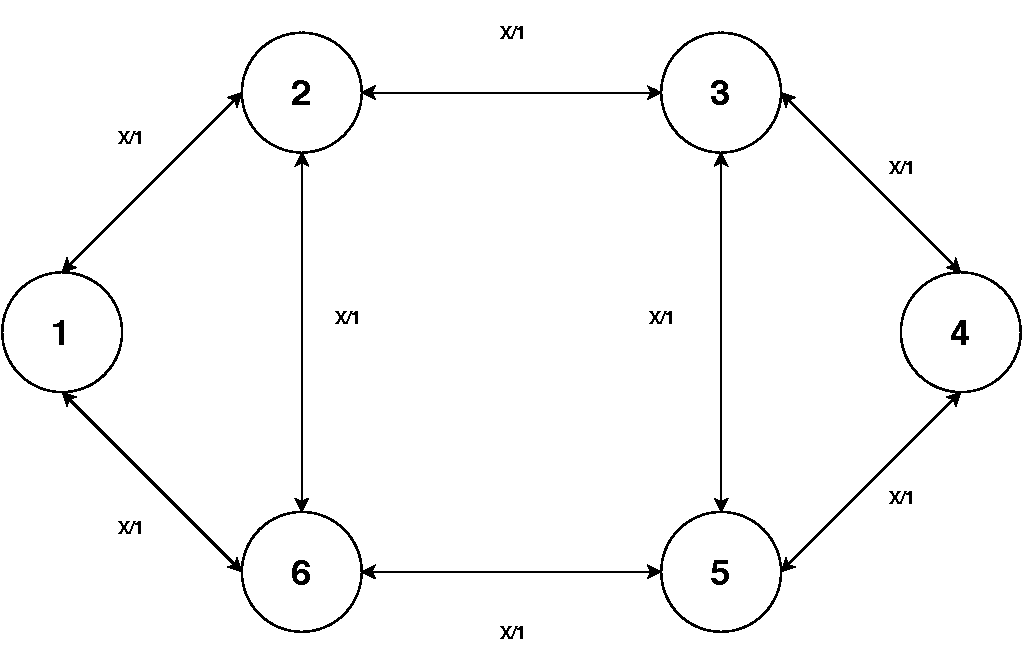
\includegraphics[width=0.7\textwidth]{fig/logos/physicalTopology.pdf}
    \caption{Reference network physical topology graph representation.}
  \end{center}
   \label{referencePhysical}
\end{figure}

\begin{table}[H]
\centering
\begin{tabular}{|c|c|c|c|c|c|c|}
\hline
\textbf{Node} & \textbf{1} & \textbf{2} & \textbf{3} & \textbf{4} & \textbf{5} & \textbf{6} \\ \hline
\textbf{1} & 0 & 1 & 0 & 0 & 0 & 1 \\ \hline
\textbf{2} & 1 & 0 & 1 & 0 & 0 & 1 \\ \hline
\textbf{3} & 0 & 1 & 0 & 1 & 1 & 0 \\ \hline
\textbf{4} & 0 & 0 & 1 & 0 & 1 & 0 \\ \hline
\textbf{5} & 0 & 0 & 1 & 1 & 0 & 1 \\ \hline
\textbf{6} & 1 & 1 & 0 & 0 & 1 & 0 \\ \hline
\end{tabular}
\caption{Reference network physical topology adjacency matrix.}
\label{referenceAdjacency}
\end{table}

Above in figure \ref{referencePhysical} and table \ref{referenceAdjacency} the physical topology of the reference network is specified as a graph and in an adjacency matrix, respectively. Below we have the distance matrix that contains the actual values of distance, expressed in kilometers (km), between node sites. The values will remain the same for every traffic scenario tested and the traffic matrix must be symmetric.  
\[
Dist=
  \begin{bmatrix}
    0 & 350 & 0 & 0 & 0 & 150 \\
    350 & 0 & 350 & 0 & 0 & 150 \\
    0 & 350 & 0 & 250 & 50 & 0 \\
    0 & 0 & 250 & 0 & 150 & 0 \\
    0 & 0 & 50 & 150 & 0 & 550 \\
    150 & 150 & 0 & 0 & 550 & 0
  \end{bmatrix}
\]


In table \ref{table_ref_net1} we have the global variables that characterize the reference network.

\begin{table}[H]
\centering
\begin{tabular}{| c | c | c|}
 \hline
 Constant & Description & Value \\
 \hline\hline
 N & Number of nodes & 6 \\
 L & Number of bidirectional links & 8 \\
 <$\delta$> & Node degree & 2.667 \\
 <len> & Mean link length (km) & 250 \\
 <h> & Mean number of hops for working paths & 1.533 \\
 <h'> & Mean number of hops for backup paths & 2.467 \\
 \hline
\end{tabular}
\caption{Table of reference network values.}
\label{table_ref_net1}
\end{table}

\subsection{Logical Topology}

The logical topology of a network depends directly of the transport mode used.
\vspace{15pt}
\begin{figure}[H]
  \begin{center}
    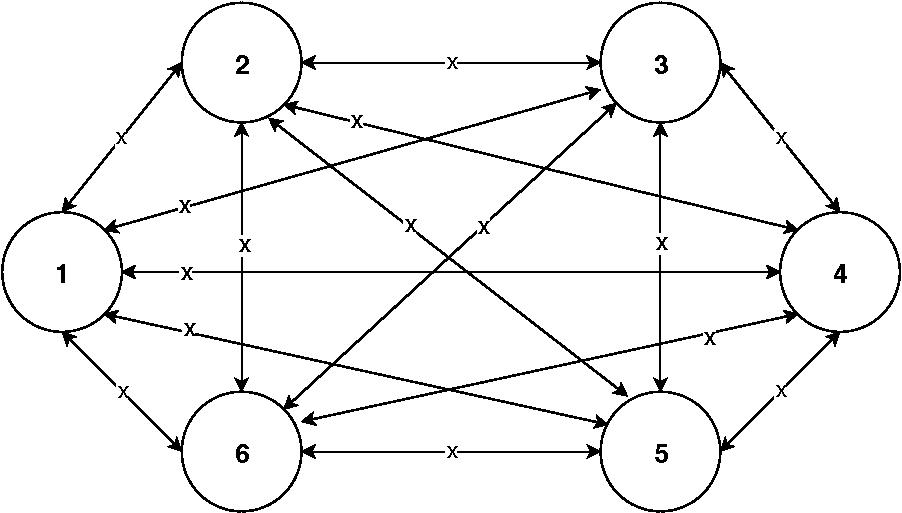
\includegraphics[width=0.7\textwidth]{fig/logos/logicalTopologyReference.pdf}
    \caption{Reference network logical topology graph representation.}
  \end{center}
   \label{referenceLogical}
\end{figure}
\clearpage
For this specific case, as only the transparent transport mode is considered, the resultant logical topology is represented in figure \ref{referenceLogical}. Like the previous, it is comprised of the same 6 nodes which in this case are directly connected, on an upper logical layer, to every other node.

\subsection{Traffic Matrices}

Three different scenarios of traffic (low, medium and high) were designed in order to better understand the later results. Each of the scenarios are composed of 5 matrices of different \gls{odu} frame types, namely, the ODU0 corresponding to 1.25 Gbit/s, the ODU1 corresponding to 2.5 Gbit/s, the ODU2 corresponding to 10 Gbit/s, the ODU3 corresponding to 40 Gbit/s and finally the ODU4 thaht corresponds to 100 Gbit/s. The matrices for all cases are symmetric, meaning that the traffic sent, for example, from node 1 to node 2 is the same as the traffic sent from node 2 to 1. Since in this case all the traffic requests are known the network traffic is said to be static.

\subsubsection{Low Traffic Scenario}
\label{low}

In this case, it was chosen to have a total unidirectional traffic of 2 Tbit/s. That amount of traffic was distributed through the different ODU type matrices as it can be seen below. 
\[
ODU0=
  \begin{bmatrix}
    0 & 10 & 2 & 6 & 2 & 6 \\
    10 & 0 & 0 & 2 & 10 & 0 \\
    2 & 0 & 0 & 2 & 8 & 2 \\
    6 & 2 & 2 & 0 & 2 & 2 \\
    2 & 10 & 8 & 2 & 0 & 6 \\
    6 & 0 & 2 & 2 & 6 & 0
  \end{bmatrix}
\qquad ODU1=
  \begin{bmatrix}
    0 & 4 & 8 & 4 & 0 & 10 \\
    4 & 0 & 0 & 6 & 2 & 2 \\
    8 & 0 & 0 & 2 & 2 & 0 \\
    4 & 6 & 2 & 0 & 2 & 6 \\
    0 & 2 & 2 & 2 & 0 & 2 \\
    10 & 2 & 0 & 6 & 2 & 0
  \end{bmatrix}
\]
\[
ODU2=
  \begin{bmatrix}
    0 & 2 & 2 & 2 & 0 & 0 \\
    2 & 0 & 0 & 0 & 2 & 0 \\
    2 & 0 & 0 & 2 & 2 & 0 \\
    2 & 0 & 2 & 0 & 2 & 0 \\
    0 & 2 & 2 & 2 & 0 & 2 \\
    0 & 0 & 0 & 0 & 2 & 0
  \end{bmatrix}
\qquad ODU3=
  \begin{bmatrix}
    0 & 0 & 0 & 0 & 0 & 0 \\
    0 & 0 & 2 & 0 & 0 & 2 \\
    0 & 2 & 0 & 0 & 2 & 0 \\
    0 & 0 & 0 & 0 & 0 & 0 \\
    0 & 0 & 2 & 0 & 0 & 0 \\
    0 & 2 & 0 & 0 & 0 & 0
  \end{bmatrix}
\]
\[
ODU4=
  \begin{bmatrix}
    0 & 0 & 0 & 0 & 0 & 0 \\
    0 & 0 & 0 & 0 & 0 & 2 \\
    0 & 0 & 0 & 0 & 0 & 0 \\
    0 & 0 & 0 & 0 & 0 & 0 \\
    0 & 0 & 0 & 0 & 0 & 2 \\
    0 & 2 & 0 & 0 & 2 & 0
  \end{bmatrix}
\]
Through these matrices it becomes possible to calculate the total network traffic for the low traffic scenario:\\ 
$T_1^0$ = 120x1.25 = 150 Gbits/s \  $T_1^1$ = 100x2.5 = 250 Gbits/s \  $T_1^2$ = 32x10 = 320 Gbits/s \\

$T_1^3$ = 12x40 = 480 Gbits/s \quad
$T_1^4$ = 8x100 = 800 Gbits/s \\

$T_{1}$ = 150 + 250 + 320 + 480 + 800 = 2000 Gbits/s \qquad
$T$ = 1000/2 = \textbf{1 Tbits/s}\\

Where the variable $T_1^x$ represents the unidirectional traffic of the ODUx, for example, $T_1^0$ represents the unidirectional traffic of the ODU0 and $T_1^1$ represents the unidirectional traffic of the ODU1. The variable $T_{1}$ represents the total of unidirectional traffic that is injected into the network. Finally, the variable $T$ represents the total of bidirectional traffic.

\subsubsection{Medium Traffic Scenario}
\label{medium}
In this case it was chosen to have a total unidirectional traffic of 10 Tbit/s. That amount of traffic was distributed through the different ODU type matrices as it can be seen below. 

\[
ODU0=
  \begin{bmatrix}
    0 & 50 & 10 & 30 & 10 & 30 \\
    50 & 0 & 0 & 10 & 50 & 0 \\
    10 & 0 & 0 & 10 & 40 & 10 \\
    30 & 10 & 10 & 0 & 10 & 10 \\
    10 & 50 & 40 & 10 & 0 & 30 \\
    30 & 0 & 10 & 10 & 30 & 0
  \end{bmatrix}
\quad ODU1=
  \begin{bmatrix}
    0 & 20 & 40 & 20 & 0 & 50 \\
    20 & 0 & 0 & 30 & 10 & 10 \\
    40 & 0 & 0 & 10 & 10 & 0 \\
    20 & 30 & 10 & 0 & 10 & 30 \\
    0 & 10 & 10 & 10 & 0 & 10 \\
    50 & 10 & 0 & 30 & 10 & 0
  \end{bmatrix}
\]
\[
ODU2=
  \begin{bmatrix}
    0 & 10 & 10 & 10 & 0 & 0 \\
    10 & 0 & 0 & 0 & 10 & 0 \\
    10 & 0 & 0 & 10 & 10 & 0 \\
    10 & 0 & 10 & 0 & 10 & 0 \\
    0 & 10 & 10 & 10 & 0 & 10 \\
    0 & 0 & 0 & 0 & 10 & 0
  \end{bmatrix}
\quad ODU3=
  \begin{bmatrix}
    0 & 0 & 0 & 0 & 0 & 0 \\
    0 & 0 & 10 & 0 & 0 & 10 \\
    0 & 10 & 0 & 0 & 10 & 0 \\
    0 & 0 & 0 & 0 & 0 & 0 \\
    0 & 0 & 10 & 0 & 0 & 0 \\
    0 & 10 & 0 & 0 & 0 & 0
  \end{bmatrix}
\]
\[
ODU4=
  \begin{bmatrix}
    0 & 0 & 0 & 0 & 0 & 0 \\
    0 & 0 & 0 & 0 & 0 & 10 \\
    0 & 0 & 0 & 0 & 0 & 0 \\
    0 & 0 & 0 & 0 & 0 & 0 \\
    0 & 0 & 0 & 0 & 0 & 10 \\
    0 & 10 & 0 & 0 & 10 & 0
  \end{bmatrix}
\]


\vspace{17pt}
Through these matrices it becomes possible to calculate the total network traffic for the medium traffic scenario:\\

$T_1^0$ = 600x1.25 = 750 Gbits/s \  $T_1^1$ = 500x2.5 = 1205 Gbits/s \  $T_1^2$ = 160x10 = 1600 Gbits/s \\

$T_1^3$ = 60x40 = 2400 Gbits/s \quad
$T_1^4$ = 40x100 = 4000 Gbits/s \\

$T_{1}$ = 750 + 1250 + 1600 + 2400 + 4000 = 10000 Gbits/s \qquad
$T$ = 10000/2 = \textbf{5 Tbits/s}\\



\subsubsection{High Traffic Scenario}
\label{high}
In this case it was chosen to have a total unidirectional traffic of 20 Tbit/s. That amount of traffic was distributed through the different ODU type matrices as it can be seen below. 
\[
ODU0=
  \begin{bmatrix}
    0 & 100 & 20 & 60 & 20 & 60 \\
    100 & 0 & 0 & 20 & 100 & 0 \\
    20 & 0 & 0 & 20 & 80 & 20 \\
    60 & 20 & 20 & 0 & 20 & 20 \\
    20 & 100 & 80 & 20 & 0 & 60 \\
    60 & 0 & 20 & 20 & 60 & 0
  \end{bmatrix}
\quad ODU1=
  \begin{bmatrix}
    0 & 40 & 80 & 40 & 0 & 100 \\
    40 & 0 & 0 & 60 & 20 & 20 \\
    80 & 0 & 0 & 20 & 20 & 0 \\
    40 & 60 & 20 & 0 & 20 & 60 \\
    0 & 20 & 20 & 20 & 0 & 20 \\
    100 & 20 & 0 & 60 & 20 & 0
  \end{bmatrix}
\]
\[
ODU2=
  \begin{bmatrix}
    0 & 20 & 20 & 20 & 0 & 0 \\
    20 & 0 & 0 & 0 & 20 & 0 \\
    20 & 0 & 0 & 20 & 20 & 0 \\
    20 & 0 & 20 & 0 & 20 & 0 \\
    0 & 20 & 20 & 20 & 0 & 20 \\
    0 & 0 & 0 & 0 & 20 & 0
  \end{bmatrix}
\quad ODU3=
  \begin{bmatrix}
    0 & 0 & 0 & 0 & 0 & 0 \\
    0 & 0 & 20 & 0 & 0 & 20 \\
    0 & 20 & 0 & 0 & 20 & 0 \\
    0 & 0 & 0 & 0 & 0 & 0 \\
    0 & 0 & 20 & 0 & 0 & 0 \\
    0 & 20 & 0 & 0 & 0 & 0
  \end{bmatrix}
\]
\[
ODU4=
  \begin{bmatrix}
    0 & 0 & 0 & 0 & 0 & 0 \\
    0 & 0 & 0 & 0 & 0 & 20 \\
    0 & 0 & 0 & 0 & 0 & 0 \\
    0 & 0 & 0 & 0 & 0 & 0 \\
    0 & 0 & 0 & 0 & 0 & 20 \\
    0 & 20 & 0 & 0 & 20 & 0
  \end{bmatrix}
\]

\vspace{17pt}
Through these matrices it becomes possible to calculate the total network traffic for the high traffic scenario:

$T_1^0$ = 1200x1.25 = 1500 Gbits/s \qquad
$T_1^1$ = 1000x2.5 = 2500 Gbits/s \\

$T_1^2$ = 320x10 = 3200 Gbits/s \qquad
$T_1^3$ = 120x40 = 4800 Gbits/s \\

$T_1^4$ = 80x100 = 8000 Gbits/s \qquad
$T_{1}$ = 20000 Gbits/s \\

$T$ = 20000/2 = \textbf{10 Tbits/s}



\section{Realistic Network}
\label{realisticNetwork}

The nodes are geographically distributed as shown in figure \ref{vbns}. As it can be seen this network is composed of 12 nodes and 17 bidirectional links.
\begin{figure}[H]
  \label{cisco}
  \begin{center}
    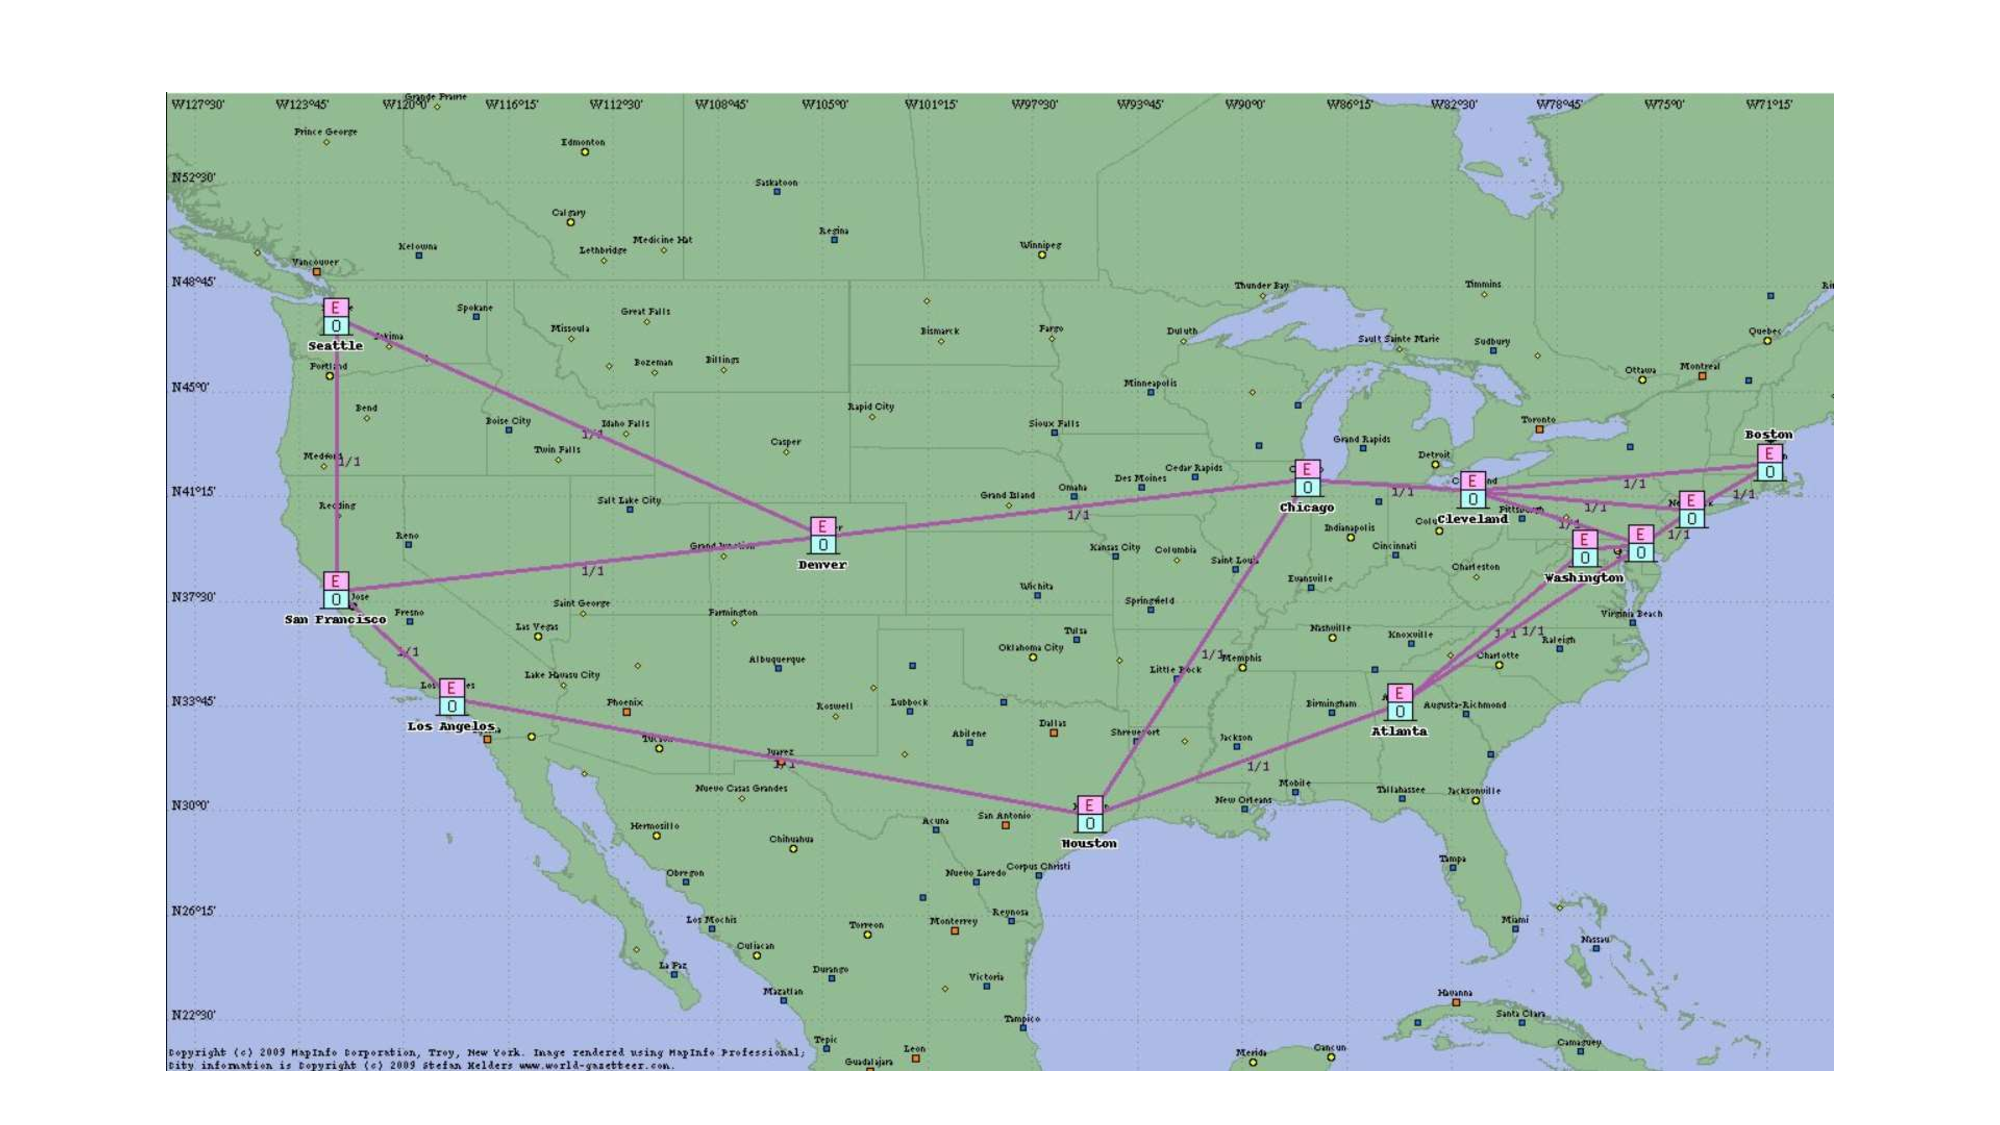
\includegraphics[width=1\textwidth]{fig/logos/realisticNetwork.pdf}
    \caption{The Very-High Performance Backbone Network Service \cite{redeRealista}.}
  \end{center}
  \label{vbns}
\end{figure}

In order to validate the developed heuristic algorithms it was decided to apply them into a real and more complex network. The chosen network was the vBNS (very high-speed Backbone Network Service), which is a National Science Foundation sponsored high-performance network service implemented in the United States of America by the MCI Telecommunications Corporation. It supports scientific applications between NSF-supported supercomputer centers, directly connected research institutions and research institutions that are served by other networks \cite{568211}. As before the only the transparent transport mode without survivability will be approached.

\subsection{Physical Topology}


\begin{figure}[H]
  \begin{center}
    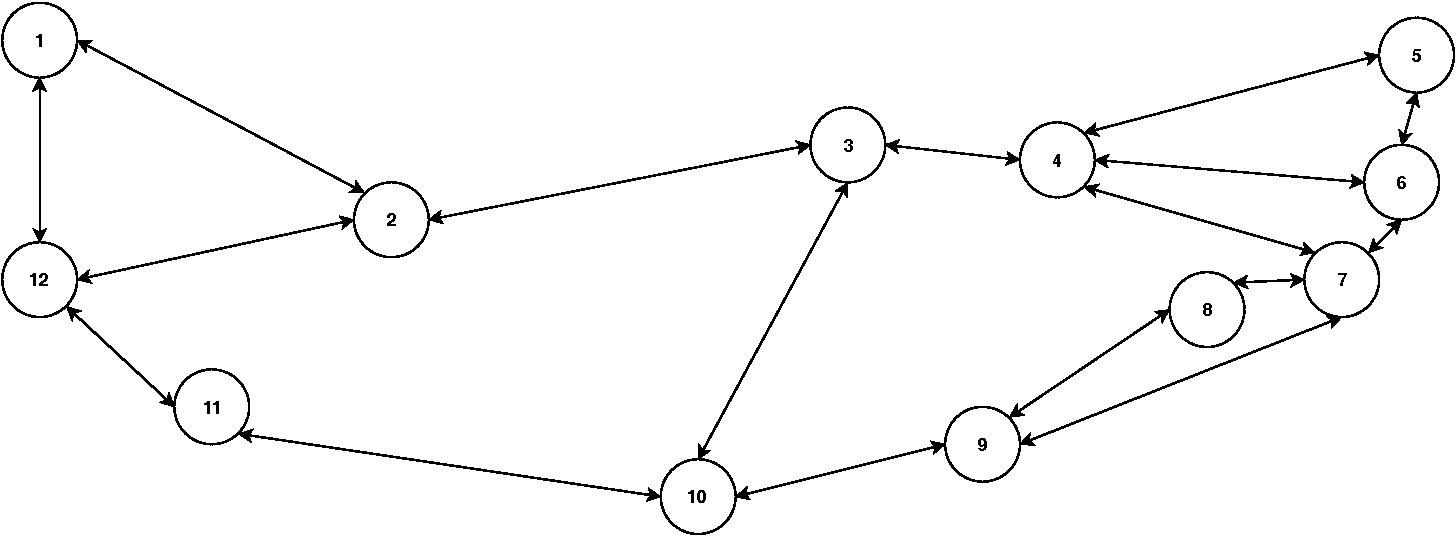
\includegraphics[width=0.9\textwidth]{fig/logos/vBNS.pdf}
    \caption{Physical topology graph representation.}
  \end{center}
  \label{rptg}
\end{figure}

\begin{table}[H]
\centering
\begin{tabular}{|c|c|c|c|c|c|c|c|c|c|c|c|c|}
\hline
\textbf{Node} & \textbf{1} & \textbf{2} & \textbf{3} & \textbf{4} & \textbf{5} & \textbf{6} & \textbf{7} & \textbf{8} & \textbf{9} & \textbf{10} & \textbf{11} & \textbf{12} \\ \hline
\textbf{1} & 0 & 1 & 0 & 0 & 0 & 0 & 0 & 0 & 0 & 0 & 0 & 1 \\ \hline
\textbf{2} & 1 & 0 & 1 & 0 & 0 & 0 & 0 & 0 & 0 & 0 & 0 & 1 \\ \hline
\textbf{3} & 0 & 1 & 0 & 1 & 0 & 0 & 0 & 0 & 0 & 1 & 0 & 0 \\ \hline
\textbf{4} & 0 & 0 & 1 & 0 & 1 & 1 & 1 & 0 & 0 & 0 & 0 & 0 \\ \hline
\textbf{5} & 0 & 0 & 0 & 1 & 0 & 1 & 0 & 0 & 0 & 0 & 0 & 0 \\ \hline
\textbf{6} & 0 & 0 & 0 & 1 & 1 & 0 & 1 & 0 & 0 & 0 & 0 & 0 \\ \hline
\textbf{7} & 0 & 0 & 0 & 1 & 0 & 1 & 0 & 1 & 1 & 0 & 0 & 0 \\ \hline
\textbf{8} & 0 & 0 & 0 & 0 & 0 & 0 & 1 & 0 & 1 & 0 & 0 & 0 \\ \hline
\textbf{9} & 0 & 0 & 0 & 0 & 0 & 0 & 1 & 1 & 0 & 1 & 0 & 0 \\ \hline
\textbf{10} & 0 & 0 & 1 & 0 & 0 & 0 & 0 & 0 & 1 & 0 & 1 & 0 \\ \hline
\textbf{11} & 0 & 0 & 0 & 0 & 0 & 0 & 0 & 0 & 0 & 1 & 0 & 1 \\ \hline
\textbf{12} & 1 & 1 & 0 & 0 & 0 & 0 & 0 & 0 & 0 & 0 & 1 & 0 \\ \hline
\end{tabular}
\caption{Physical topology adjacency matrix.}
\label{rptam}
\end{table}

Above in figure \ref{rptg} and table \ref{rptam} the physical topology of the realistic network is specified as a graph and in an adjacency matrix, respectively. 

In table \ref{table_ref_net} we have the global variables that characterize the Very-High Performance Backbone Network Service.

\begin{table}[H]
\centering
\begin{tabular}{| c | c | c|}
 \hline
 Constant & Description & Value \\
 \hline\hline
 N & Number of nodes & 12 \\
 L & Number of bidirectional links & 17 \\
 <$\delta$> & Node degree & 2.83 \\
 <len> & Mean link length (km) & 965 \\
 <h> & Mean number of hops for working paths & 2.40 \\
 <h'> & Mean number of hops for backup paths & 3.90 \\
 \hline
\end{tabular}
\caption{Table of vBNS network values.}
\label{table_ref_net}
\end{table}


\subsection{Traffic Matrices}
\label{referenceTraffic}
Below, are presented the traffic matrices used in order to test this network. The matrices for this traffic scenario were generated randomly. The total amount of bidirectional traffic in the network considering this set of demands stays around 7.5 Tbit/s. It should be noted that the total number of columns and rows is equal to the number of nodes and the main diagonal of the matrices is composed of zeros, since it does not make sense for a node to send traffic to itself. Additionally, the missing matrices for ODU0 and ODU4 represent the absence of demand requests of this type.  %depois explicar o porquê
\vspace{11pt}

\begin{table}[H]
\centering
\begin{tabular}{|c|c|c|c|c|c|c|c|c|c|c|c|c|}
\hline
\textbf{ODU1} & 1 & 2 & 3 & 4 & 5 & 6 & 7 & 8 & 9 & 10 & 11 & 12 \\ \hline
1 & 0 & 0 & 2 & 4 & 4 & 3 & 1 & 3 & 4 & 0 & 0 & 0 \\ \hline
2 & 0 & 0 & 50 & 5 & 50 & 5 & 5 & 50 & 5 & 0 & 5 & 50 \\ \hline
3 & 2 & 50 & 0 & 5 & 5 & 5 & 5 & 5 & 5 & 5 & 5 & 50 \\ \hline
4 & 4 & 5 & 5 & 0 & 4 & 6 & 0 & 0 & 0 & 1 & 30 & 2 \\ \hline
5 & 4 & 50 & 5 & 4 & 0 & 1 & 6 & 3 & 3 & 6 & 9 & 3 \\ \hline
6 & 3 & 5 & 5 & 6 & 1 & 0 & 1 & 6 & 4 & 6 & 3 & 2 \\ \hline
7 & 1 & 5 & 5 & 0 & 6 & 1 & 0 & 2 & 3 & 9 & 2 & 2 \\ \hline
8 & 3 & 50 & 5 & 0 & 3 & 6 & 2 & 0 & 3 & 6 & 3 & 1 \\ \hline
9 & 4 & 5 & 5 & 0 & 3 & 4 & 3 & 3 & 0 & 40 & 3 & 2 \\ \hline
10 & 0 & 0 & 5 & 1 & 6 & 6 & 9 & 6 & 40 & 0 & 9 & 3 \\ \hline
11 & 0 & 5 & 5 & 30 & 9 & 3 & 2 & 3 & 3 & 9 & 0 & 1 \\ \hline
12 & 0 & 50 & 50 & 2 & 3 & 2 & 2 & 1 & 2 & 3 & 1 & 0 \\ \hline
\end{tabular}
\caption{ODU1 traffic matrix for the realistic network.}
\label{referenceODU1}
\end{table}

Through table \ref{referenceODU1} is possible to obtain the quantity of unidirectional ODU1 traffic in the network:

$T_1^1$ = 394x2.5 = 985 Gbits/s \qquad
\vspace{11pt}
\begin{table}[H]
\centering
\begin{tabular}{|c|c|c|c|c|c|c|c|c|c|c|c|c|}
\hline
\textbf{ODU2} & 1 & 2 & 3 & 4 & 5 & 6 & 7 & 8 & 9 & 10 & 11 & 12 \\ \hline
1 & 0 & 0 & 0 & 0 & 0 & 0 & 0 & 0 & 1 & 2 & 1 & 1 \\ \hline
2 & 0 & 0 & 2 & 2 & 1 & 1 & 2 & 1 & 2 & 2 & 1 & 1 \\ \hline
3 & 0 & 2 & 0 & 1 & 2 & 2 & 4 & 1 & 0 & 0 & 0 & 2 \\ \hline
4 & 0 & 2 & 1 & 0 & 2 & 4 & 2 & 1 & 2 & 2 & 0 & 2 \\ \hline
5 & 0 & 1 & 2 & 2 & 0 & 2 & 2 & 0 & 0 & 0 & 1 & 4 \\ \hline
6 & 0 & 1 & 2 & 4 & 2 & 0 & 2 & 4 & 2 & 1 & 2 & 1 \\ \hline
7 & 0 & 2 & 4 & 2 & 2 & 2 & 0 & 4 & 1 & 0 & 0 & 0 \\ \hline
8 & 0 & 1 & 1 & 1 & 0 & 4 & 4 & 0 & 1 & 2 & 2 & 2 \\ \hline
9 & 1 & 2 & 0 & 2 & 0 & 2 & 1 & 1 & 0 & 4 & 2 & 2 \\ \hline
10 & 2 & 2 & 0 & 2 & 0 & 1 & 0 & 2 & 4 & 0 & 1 & 4 \\ \hline
11 & 1 & 1 & 0 & 0 & 1 & 2 & 0 & 2 & 2 & 1 & 0 & 2 \\ \hline
12 & 1 & 1 & 2 & 2 & 4 & 1 & 0 & 2 & 2 & 4 & 2 & 0 \\ \hline
\end{tabular}
\caption{ODU2 traffic matrix for the realistic network.}
\label{referenceODU2}
\end{table}

Through table \ref{referenceODU2} is possible to obtain the quantity of unidirectional ODU2 traffic in the network:

$T_1^2$ = 190x10 = 1 900 Gbits/s \qquad
\vspace{11pt}
\begin{table}[H]
\centering
\begin{tabular}{|c|c|c|c|c|c|c|c|c|c|c|c|c|}
\hline
\textbf{ODU3} & 1 & 2 & 3 & 4 & 5 & 6 & 7 & 8 & 9 & 10 & 11 & 12 \\ \hline
1 & 0 & 5 & 1 & 2 & 2 & 0 & 2 & 2 & 5 & 5 & 5 & 0 \\ \hline
2 & 5 & 0 & 1 & 10 & 1 & 10 & 2 & 2 & 2 & 2 & 2 & 2 \\ \hline
3 & 1 & 1 & 0 & 1 & 2 & 20 & 2 & 2 & 2 & 0 & 2 & 0 \\ \hline
4 & 2 & 10 & 1 & 0 & 2 & 1 & 1 & 2 & 2 & 1 & 4 & 1 \\ \hline
5 & 2 & 1 & 2 & 2 & 0 & 0 & 0 & 2 & 1 & 1 & 4 & 0 \\ \hline
6 & 0 & 10 & 20 & 1 & 0 & 0 & 2 & 1 & 4 & 4 & 1 & 2 \\ \hline
7 & 2 & 2 & 2 & 1 & 0 & 2 & 0 & 2 & 4 & 2 & 2 & 2 \\ \hline
8 & 2 & 2 & 2 & 2 & 2 & 1 & 2 & 0 & 2 & 1 & 4 & 2 \\ \hline
9 & 5 & 2 & 2 & 2 & 1 & 4 & 4 & 2 & 0 & 1 & 2 & 4 \\ \hline
10 & 5 & 2 & 0 & 1 & 1 & 4 & 2 & 1 & 1 & 0 & 1 & 1 \\ \hline
11 & 5 & 2 & 2 & 4 & 4 & 1 & 2 & 4 & 2 & 1 & 0 & 5 \\ \hline
12 & 0 & 2 & 0 & 1 & 0 & 2 & 2 & 2 & 4 & 1 & 5 & 0 \\ \hline
\end{tabular}
\caption{ODU3 traffic matrix for the realistic network.}
\label{referenceODU3}
\end{table}

Through table \ref{referenceODU3} is possible to obtain the quantity of unidirectional ODU3 traffic in the network:

$T_1^3$ = 314x40 = 12 560 Gbits/s \qquad \\

\vspace{11pt}
$T_{1}$ = 0 + 985 + 1 900 + 12 560 + 0 $\sim$ 15 Tbits/s \qquad

$T$ = 1000/2 = \textbf{7.5 Tbits/s}\\

Once again, as referred in the previous section the variable $T_1^x$ represents the unidirectional traffic of the ODUx, for example, $T_1^0$ represents the unidirectional traffic of the ODU0 and $T_1^1$ represents the unidirectional traffic of the ODU1. The variable $T_{1}$ represents the total of unidirectional traffic that is injected into the network. Finally, the variable $T$ represents the total of bidirectional traffic.

\section{Chapter summary}
\vspace{11pt}
An optical network is mainly composed of fiber-optic cables that carry channels of light, combined with the equipment deployed along the fiber to process it \cite{SimmonsJane2008}. The two main concepts in optical network designing are the physical and logical topologies of the network, on which directly depend their capabilities. The layout of the network, i.e., the physical locations of the node sites and connections between them define the physical topology, on the other hand, the logical topology represents an upper layer that defines how the elements of the network may be optically connected between each other, and as such, different logical topologies are related to how the optical signal can propagate in the network \cite{Vasco}. In this dissertation only the transparent transport mode is addressed, where every node is directly connected to all others, meaning that the signal propagates from its source node to the respective destination node always in the optical domain, without suffering \gls{o-e-o} conversions and so a single-hop grooming scheme is applied. This so called optical-bypass can cause significant savings on the electrical components of a node. The calculation of the CAPEX values of a network can be performed recurring to various methods, in this chapter was analyzed an analytical, an ILP and a heuristic model and applied to the study of both a reference and a realistic network. 

\cleardoublepage